\documentclass[conference,a4paper]{IEEEtran}
\usepackage[utf8]{inputenc}
\usepackage{graphicx}
\pagenumbering{arabic}

\usepackage{tikz}
\usepackage{tcolorbox}

\usepackage{amsmath}
\usepackage{amssymb}

\usepackage{xcolor}
\usepackage{hyperref}
\hypersetup{colorlinks=true, linkcolor=teal, urlcolor=violet, citecolor=gray}

\newcommand\mysection[1]{\section[#1]{\MakeUppercase{\textbf{#1}}}}
\newcommand\mysubsection[1]{\subsection{\textup{\textbf{#1}}}}
\newcommand\mysubsubsection[1]{\subsubsection{#1}}

\title{Modular Performance Analysis \\ Using Real-Time Calculus}
\author{Rebekka Roßberg\\Institute of Embedded Systems/ Real-Time Systems\\Ulm University\\rebekka.rossberg@uni-ulm.de}

\begin{document}
\maketitle

\thispagestyle{plain}
\pagestyle{plain}

\begin{tcolorbox}[title=Abstract]
  The system-level analysis, and therefore the optimization of embedded real-time systems, plays an important role in the design process.
One way to perform such an analysis, is by using the powerful, yet simple, framework of modular performance analysis (\textbf{MPA}), which utilizes the formal analysis methods
of real-time calculus (\textbf{RTC}) to evaluate various performance criteria of hard real-time systems.
This analysis is done by building a system performance model, which sums up all the information, that is
needed for the following performance analysis.
In this paper an overview on RTC, MPA and their use is given and illustrated by a sample system.
\end{tcolorbox}

\mysection{Introduction}\label{introduction}

%In today's life embedded real-time systems can be found pretty much everywhere you go: traffic lights, the washing machine or digital alarm clocks, they all make use of this technology.
When designing an embedded real-time system there are many questions we need to be answered already in the early stages of the design cycle: 
What architecture to choose? What scheduling to use? How powerful do the CPUs need to be? Is the performance of the underlying execution platform sufficient to fulfill the given deadlines?
These questions can be answered best by using system-level performance analysis.

In general there are different categories of approaches for evaluating embedded systems.
Above all there are holistic, simulation based and formal analysis methods for system-level performance~\cite{wan:06}.
The latter category contains the modular performance analysis based on real-time calculus, which this paper is dedicated to.

With MPA, we want to have an analysis method, that can work with only little information about the system~\cite{wan:06}.
Additionally, we need to be able to evaluate, and therefore compare, numerous possible system models within a short time.
This specifically sets the need for a short analysis time.
Furthermore, we want the analysis process to be able, to deal with all kinds of different applications, environments, resource sharing strategies and hardware platforms~\cite{thi:07},
that a distributed, heterogeneous and highly complex multiprocessor embedded real-time system might offer.
As a real-time system is defined as a system, that can always guarantee to complete its task before a given deadline~\cite{mar}, we need to know the guaranteed maximum response times of the system.
However, having completely accurate results, knowing average case response times and being able to model details, is not really important yet.

\mysubsection{About the Paper}

Initially we will characterize the system data (\autoref{data}) that is needed in order to perform the MPA and model this data using arrival and service 
curve sets in \autoref{arrivalCurves} and \autoref{serviceCurves}. 
In \autoref{complexSystem} we will build the system performance model out of HW/SW-components (\autoref{component}).
This model we are then going to analyze on performance (\autoref{performanceAnalysis}) and sensitivity (\autoref{sensitivityAnalyis}) properties, in order to find answers to important design questions regarding the embedded real-time system.
Finally, we are going to discuss (\autoref{discussion}) whether MPA really is a suitable framework for the context specified above.

While not proposing any new research, a general overview of MPA and RTC is given.
It shall be an introduction into the topic and a guide for utilizing MPA to evaluate own embedded real-time systems.
The paper is limited to the evaluation of hard real-time systems.
Those are systems, in which a single missed deadline may lead to a complete failure of the system.
Therefore, hardware and software have to operate strictly within the given time limits.

Most chapters will be accompanied by the example of an embedded real-time system. Here we will analyze, and later on optimize, the properties of a simple message-receiver device to illustrate the use of MPA.\
This example was made using the \href{https://www.mpa.ethz.ch/}{RTC Toolbox for Matlab}.
Therefore, the plots are designed using Matlab.
The example itself is constructed by myself, yet inspired by~\cite{ver}.

\mysubsection{Terminology}

First up, we want to introduce the three main concepts of this paper, along with their correlations between each other.

\textbf{Network calculus} is a ``mathematical approach to model network behavior''~\cite{thi:00} and thus an approach to model the flow of data through the network. 
It provides a general formal framework, as well as useful tools, to compute the worst case bounds on different characteristics of the communication network,
such as queuing delays and required buffer sizes~\cite{sof:12/2}.
To reveal those bounds, network calculus integrates information about the packet scheduling algorithms, the incoming events and much more~\cite{thi:00}.

When combining the results of network calculus with the theory of the min/max-plus linear system (see \autoref{minMaxPlus}) and the theory of real-time scheduling, we end up with \textbf{RTC}:
a framework, specifically designed for analyzing hard heterogeneous real-time systems~\cite{thi:00}.
Hence, most of the theorems of network calculus can now also be adapted to real-time systems.
Here the incoming event streams and available system capacities are described using curves,
which can then be transformed, whenever they are being processed at any system component.
In this way hard upper and lower bounds of the embedded real-time system's characteristics, like delays and buffers, can be computed.
The RTC framework was first proposed by~\cite{thi:00} and later on extended by the framework of MPA in~\cite{cha}.

\textbf{MPA} defines a specific, RTC based, approach to perform a system-level performance analysis of a distributed embedded real-time system.
Here ``performance'' is defined, as to what extent the system meets its answer time requirements~\cite{thi:07}.
Therefore, the performance analysis is the process of determining these properties.
To characterize end-to-end delays, response time and other system properties, MPA now cuts the system into its components in a modular way.
Afterwards all the data is combined into one big abstract system performance model, along with information about the environment, the components itself and the architecture.
This model can be analyzed now using the formal possibilities of RTC to gain insight into the system, as well as to obtain hard upper and lower bounds to various system properties~\cite{wan:05}.
\mysection{Collecting Data for Modelling the System}\label{data}

Before being able to build a system model, we must first collect some data about the application and the available resources.

\mysubsection{General Approach}

Quite little information is needed for constructing a system performance model, yet some data is fundamental for the following analysis.
What are the specifications of the incoming event streams, including their patterns, periods and deadlines?
Which of these events can occur in parallel?
(Note that this information needs to be given by formal specifications, not from observation or simulation~\cite{wan:06}.)
What resource demands do the tasks have?
How are the processing capacities and patterns of the available system resources specified?
What scheduling technique to use?

Here we can have very different degrees of detail, as sometimes we can design the new system pretty much freely, while other times we already got specific components and architectures to use given.
Yet, in case we can freely design the system, we can now just set these parameters arbitrarily and later on, for example in \autoref{sensitivityAnalyis}, optimize them.

\mysubsection{Sample System: A Simple Message Receiver} 
To illustrate the use of MPA we will design our own little embedded system.
First the requirements to this system have to be collected.
We want to construct a simple gadget that can receive messages via a signal.
Each of the messages consists out of one to 20 ASCII characters that are displayed to the device screen once the message got received.
Besides receiving messages, the device's user can also adjust the screen's brightness by pressing the ``brighter'' or the ``darker'' button.
Other functionalities will not be implemented, especially it will not be possible to compose or send any own messages.

Therefore, the system has only two use cases that can be described using UML sequence charts (see \autoref{fig:seq_brightness} and \autoref{fig:seq_message}).

\begin{figure}
    \centering
    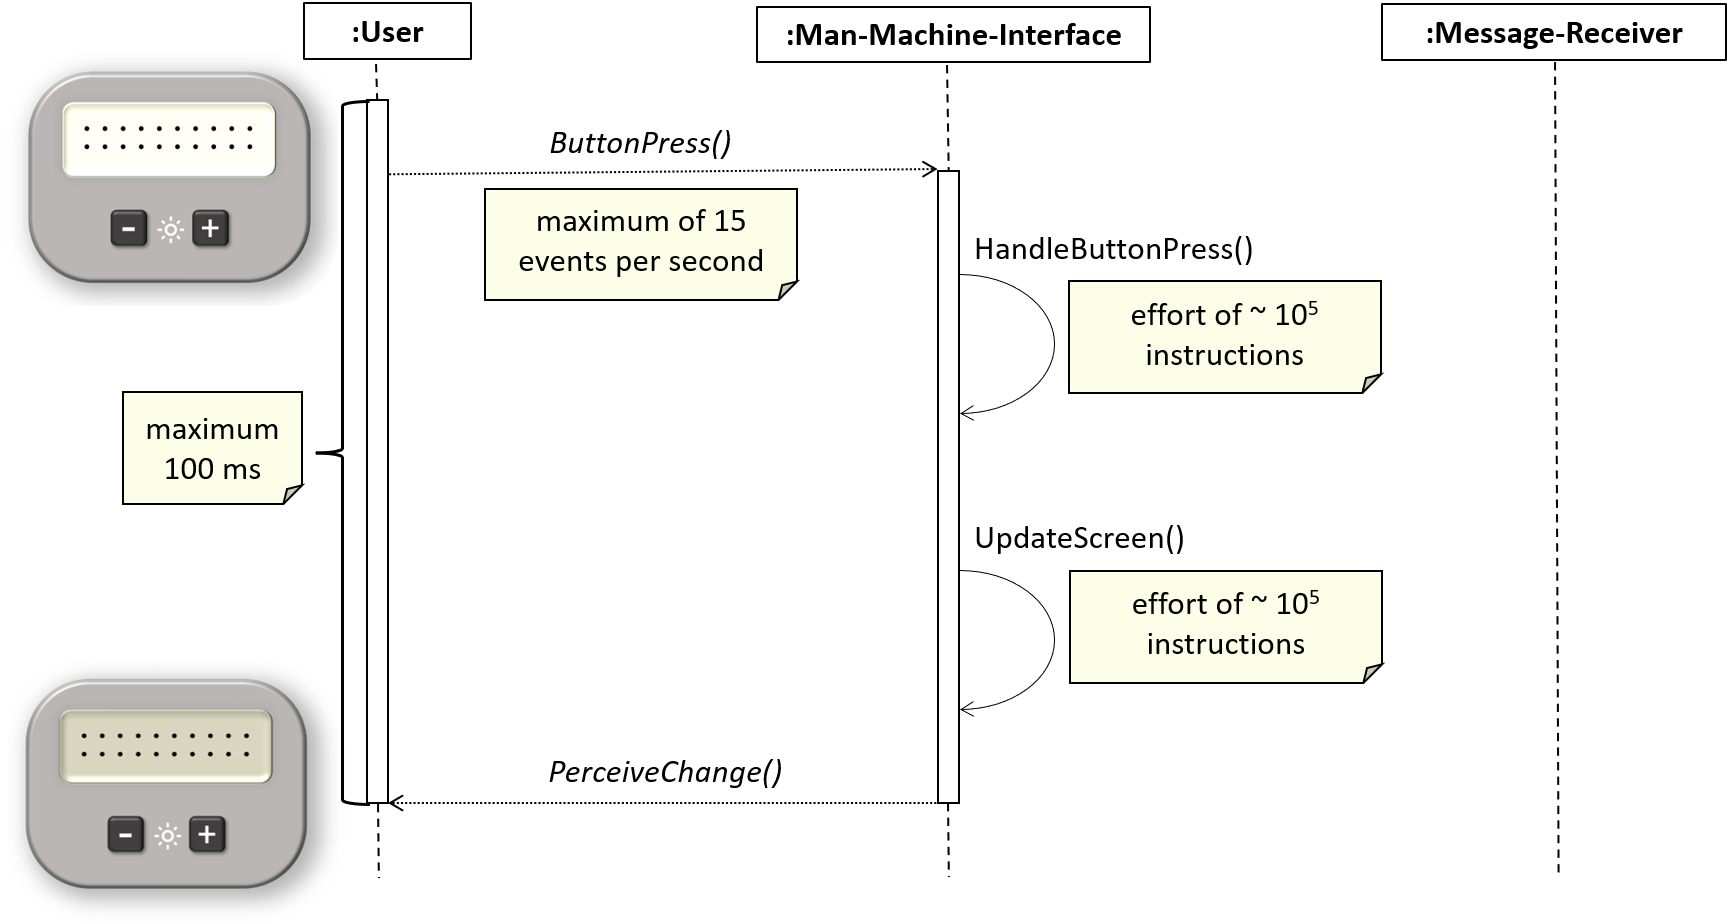
\includegraphics[width=\columnwidth]{graphics/sequence_brightness.png}
    \caption{Annotated UML Sequence Chart of the Use Case ``changing the screen's brightness''}\label{fig:seq_brightness}
\end{figure}

\begin{figure}
    \centering
    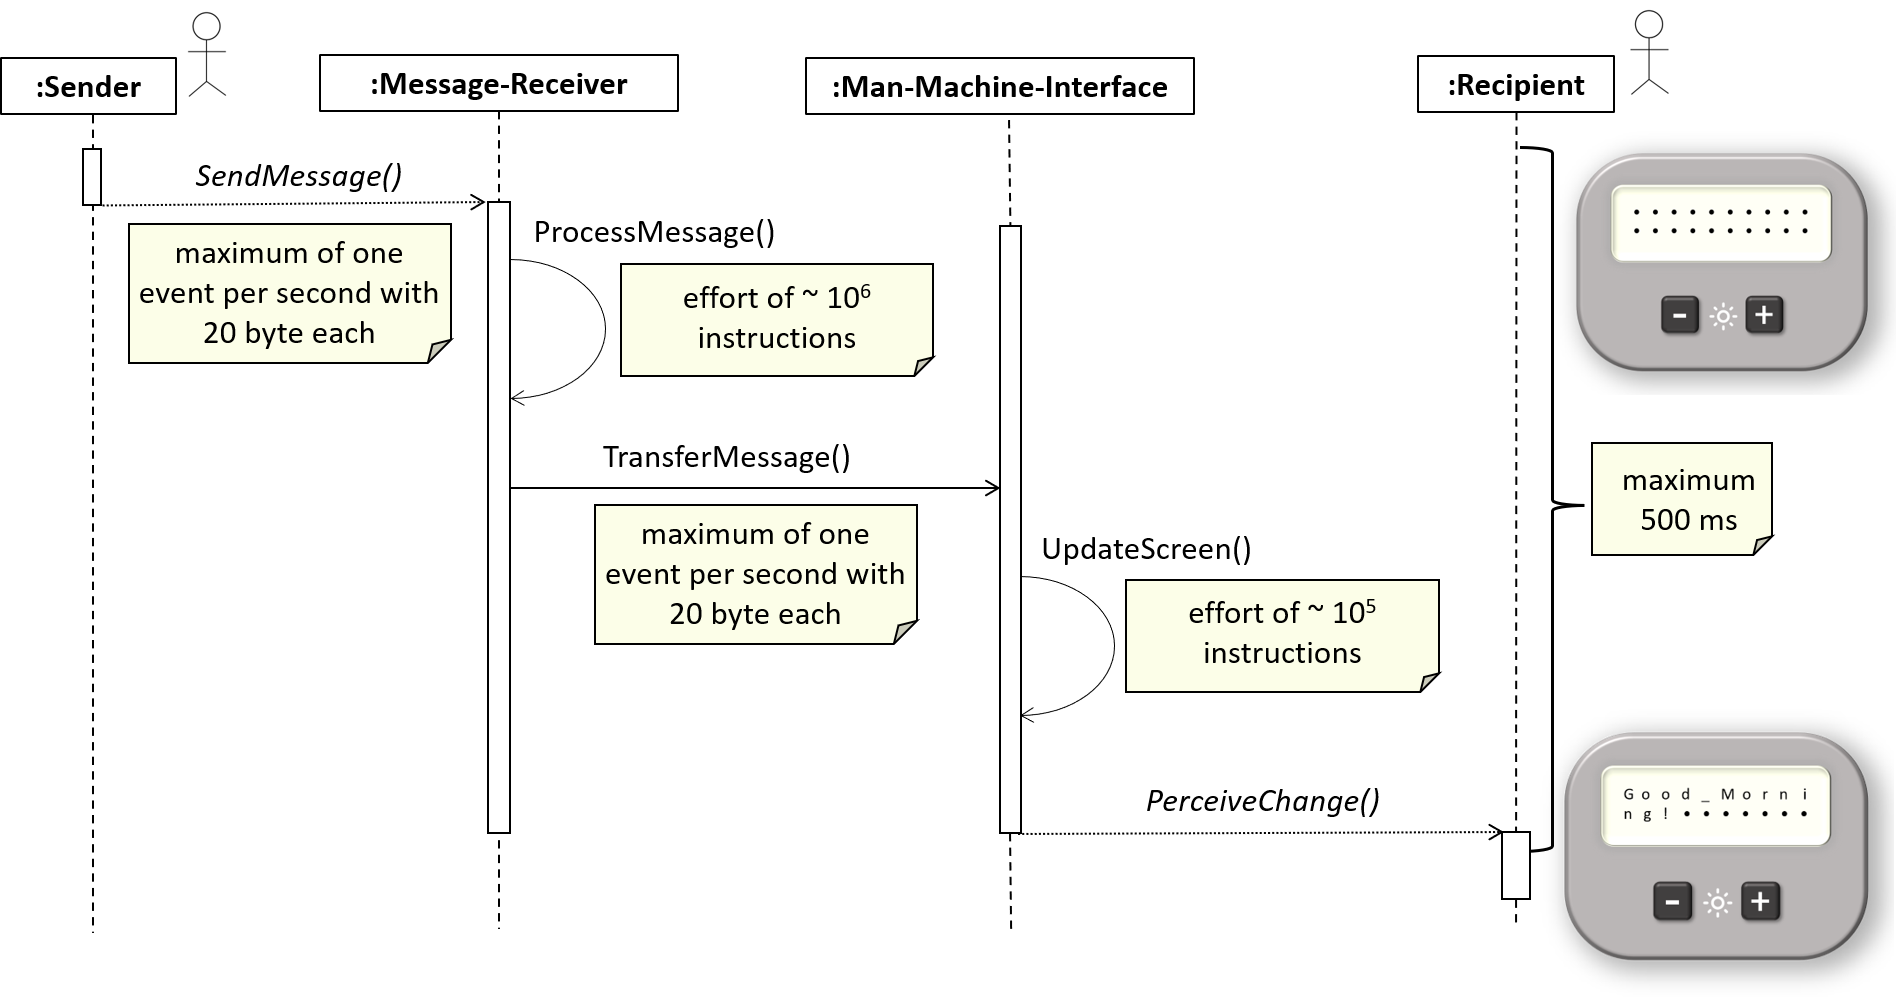
\includegraphics[width=\columnwidth]{graphics/sequence_message.png}
    \caption{Annotated UML Sequence Chart of the Use Case ``receiving a message''}\label{fig:seq_message}
\end{figure}

\mysection{Arrival Curves}\label{arrivalCurves}

Event stream models describe how a system is being used by the environment:
How often do events of a specific event stream arrive? Do these arrivals follow any kind of pattern? How much input data is provided to the system?
How much data is generated by the system and fed back to its environment after the processing~\cite{mar}?
To answer these questions, we have to construct an own event stream model for each stream of the system, by specifying the event bound functions.

\mysubsection{Event Bounds}

We define the differential arrival function \(R[s, t)\) as the total number of events that arrive within the time interval \([s, t): s,t \in \mathbb{R}\)~\cite{cho:08}.
While R models one concrete trace of an event stream, in the framework of RTC we usually characterize an event stream by its arrival curves~\cite{cho:08}:
\[\overline{\alpha}(\Delta t) = [\overline{\alpha}^{\, u}(\Delta t), \overline{\alpha}^{\, l}(\Delta t)] \]
These bounds are related by
\[\forall t \leq s \leq 0: \overline{\alpha}^{l}(t-s) \leq R[s, t) \leq \overline{\alpha}^{u}(t-s)\]
meaning that all possible traces of this event stream are located between the lower arrival curve \(\overline{\alpha}^{\, l}(\Delta t)\) and the upper arrival curve \(\overline{\alpha}^{\, u}(\Delta t)\).
Thus, these curves set guaranteed lower and upper bounds on the number of incoming events at this particular event stream over any time interval of length \(\Delta t\)~\cite{moy}.

In contrast to \(\overline{\alpha}(\Delta t)\), \(\alpha(\Delta t)\) describes the amount of resource capacity an event stream demands over a period of time\cite{cho:08}.
This specification is needed for most use cases and can be obtained by
\[[\alpha^{\, u}(\Delta t), \alpha^{\, l}(\Delta t)] = [\gamma^{u}(\overline{\alpha}^{\, u}), \gamma^{l}(\overline{\alpha}^{\, l})]\]
Here \(\gamma(e) = [\gamma^{u}(e), \gamma^{l}(e)]\) defines the minimum and maximum work, that is required per number of incoming event \textbf{e}~\cite{mar}.
Usually \(\gamma\) can be simplified to the basic linear function \(\gamma(e) = e \cdot WL\) with the task-specific workload of a single event being \textbf{WL}\cite{wan:06}.

%In more complex systems, the arriving events within one event stream may be of different types and therefore have different resource demands.
%These complex resource demands can then be modeled using automata~\cite{wan:06}.

\mysubsection{Handling Different Arrival Patterns}

Various event arrival patterns with deterministic timing behavior, such as sporadic, periodic and periodic with jitter, can be efficiently abstracted into curves~\cite{cha},~\cite{wan:12}.

In this paper we will focus on periodic event streams.
Within these streams there will always be exactly one event occurring within the period \textbf{p}.
In case we are observing a periodic event stream with a jitter \textbf{j}, that period p is guaranteed to be in \([p-j,p+j]\)~\cite{mar}.
It is important to notice, that those jitters do not accumulate: the 10th event will for example arrive within \([9p-j,10p+j]\), not within \([9p-9j,10p+10j]\).
Furthermore, the minimum distance \textbf{d} between the arrivals of two events needs to be specified whenever dealing with a jitter.

The arrival curves without jitter (\autoref{fig:simple_period}) and with jitter (\autoref{fig:period_with_jitter}) can now be modeled graphically or in the form of equations~\cite{wan:12}:
\[\overline{\alpha}^{l}(\Delta t)=\left\lfloor\frac{\Delta t-j}{p}\right\rfloor\]
\[\overline{\alpha}^{u}(\Delta t)=\min{\left\{\left\lceil\frac{\Delta t+j}{p}\right\rceil,\left\lceil\frac{\Delta t}{d}\right\rceil\right\}}\]
Those functions can also be approximated linearly to facilitate the upcoming calculations, yet this leads to less accurate results~\cite{wan:06}.

\begin{figure}
    \centering
    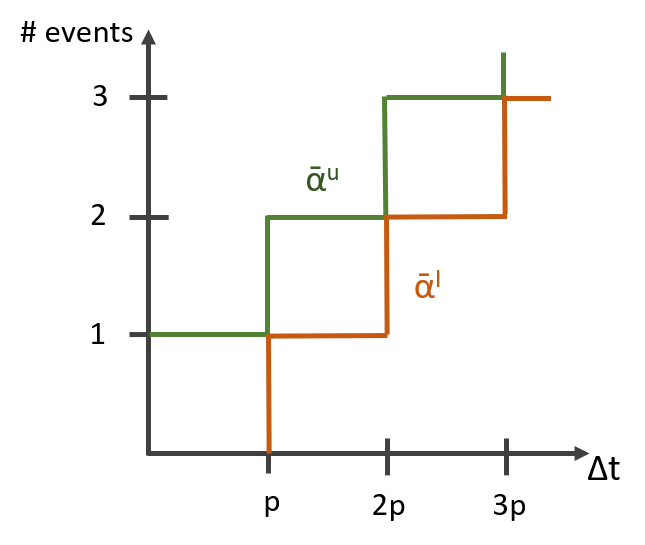
\includegraphics[width=0.7\columnwidth]{graphics/simple_period.png}
    \caption{Arrival curve with period p}\label{fig:simple_period}
\end{figure}

\begin{figure}
    \centering
    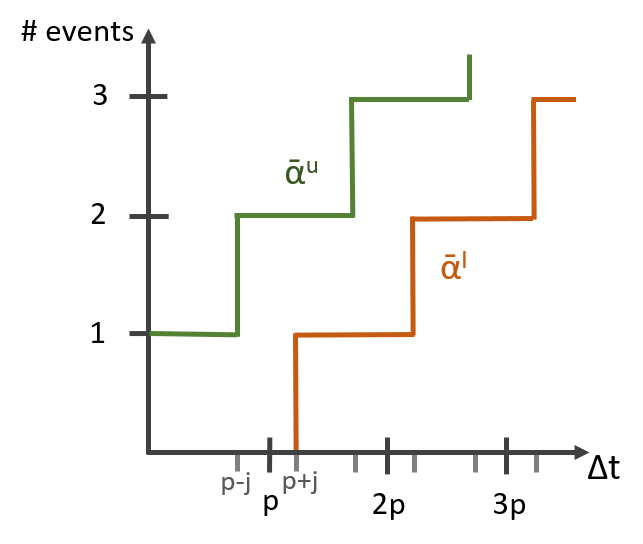
\includegraphics[width=0.7\columnwidth]{graphics/period_with_jitter.png}
    \caption{Arrival curve with period p and jitter j}\label{fig:period_with_jitter}
\end{figure}

\mysubsection{Arrival Curves of the Sample System}

As the sequence charts \autoref{fig:seq_brightness} and \autoref{fig:seq_message} define the maximum amount of incoming events per event stream and time interval,
we can easily model these streams using curves (see \autoref{fig:a-ins}).
The workload of the various tasks are also given by the sequence charts.
Therefore, we could construct the resource based arrival curves as well.

\begin{figure}
    \centering
    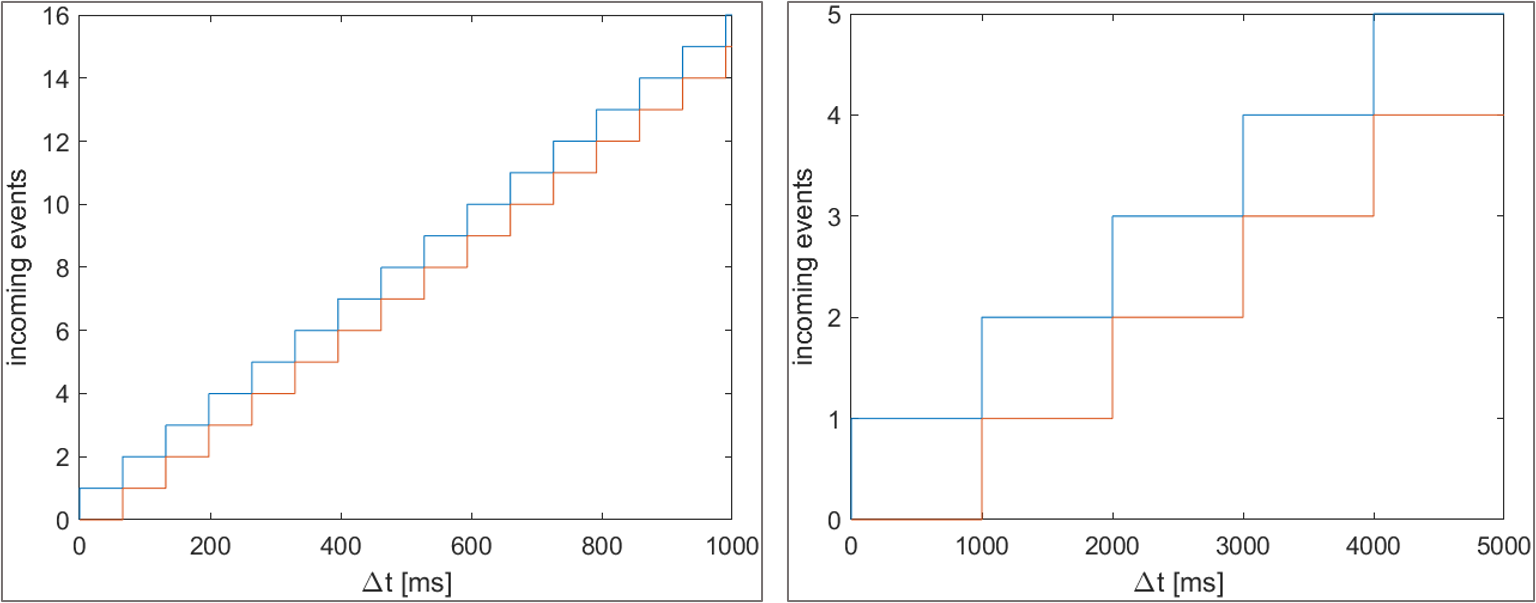
\includegraphics[width=\columnwidth]{graphics/example_a_ins.png}
    \caption{Arrival curves of brightness events (left) and message events (right)}\label{fig:a-ins}
\end{figure}
\mysection{Service Curves}\label{serviceCurves}

Resource models provide information about the processing capacities of the resources that are available within a system.
Thus, they characterize the service that can be provided by the system~\cite{mar}.
For every resource, whether communicational or computational, an own resource model has to be constructed.

\mysubsection{Resource Bounds}

We define the differential service function \(C[s, t)\) as the total number of available resource units, e.g. processor cycles or transmittable bits on a bus, within the time interval \([s, t): s,t \in \mathbb{R}\)~\cite{cho:08}.
While C models one concrete availability of a resource, in the framework of RTC we usually characterize a resource by its service curves~\cite{cho:08}:
\[\beta(\Delta t) = [\beta^{\, u}(\Delta t), \beta^{\, l}(\Delta t)]\]
The bounds are related by \[\forall t \leq s \leq 0: \beta^{l}(t-s) \leq C[s, t) \leq \beta^{u}(t-s)\]
meaning that all possible processing capacities of this component are located between the lower service curve \(\beta^{\, l}(\Delta t)\) and the upper service curve \(\beta^{\, u}(\Delta t)\).
Therefore, these curves set guaranteed lower and upper bounds on the processing units available at this resource over any time interval of length \(\Delta t\)~\cite{moy}.
In an analogue way to \(\overline{\alpha}(\Delta t)\) we can also define \(\overline{\beta}(\Delta t)\) as
\[[\overline{\beta}^{\, u}(\Delta t), \overline{\beta}^{\, l}(\Delta t)] = [(\gamma^{l})^{-1}(\beta^{\, u}), (\gamma^{u})^{-1}(\beta^{\, l})]\]
\(\overline{\beta}(\Delta t)\) directly depends on the number of events that can be processed per \(\Delta t\), yet it only has very few use cases.

\mysubsection{Handling Different Resource Availability Patterns}

The capacities of various resources, such as resources with full availability, but also with fluctuating service capacities, can be efficiently abstracted into curves~\cite{mar}.
When dealing with a simple unloaded processor with full availability, the service curve can be modeled by the linear function
\[\beta^{\, u}(\Delta t) = \beta^{\, l}(\Delta t) = APC \cdot \Delta t\] with \textbf{APC} being the constant number of available processing cycles per time interval (see \autoref{fig:simple_cpu})~\cite{mar}.

\begin{figure}
    \centering
    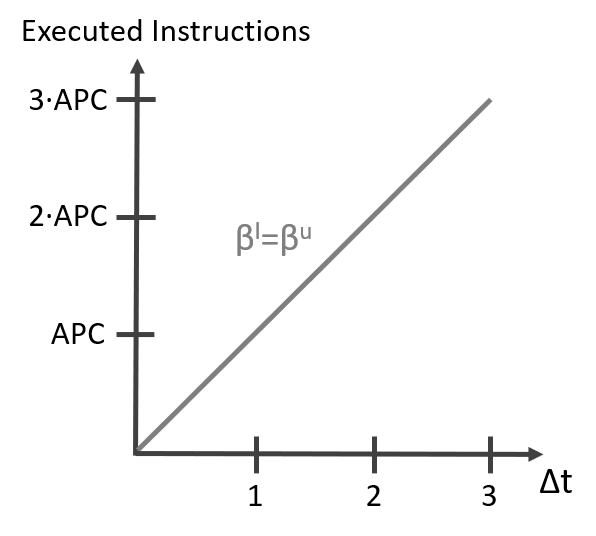
\includegraphics[width=0.6\columnwidth]{graphics/simple_cpu.png}
    \caption{Service curve of a simple CPU with full availability}\label{fig:simple_cpu}
\end{figure}

A popular example for resources with fluctuating availability are time division multiple access (\textbf{TDMA}) busses.
When communicating via a TDMA bus, information can be transmitted with a period \textbf{p} for \textbf{s} time units using the full bus bandwidth \textbf{b}.
Afterwards there is a waiting period of \(p-s\) time units until the bus gets allocated again (see \autoref{fig:tdma_bus})~\cite{mar}.

\begin{figure}
    \centering
    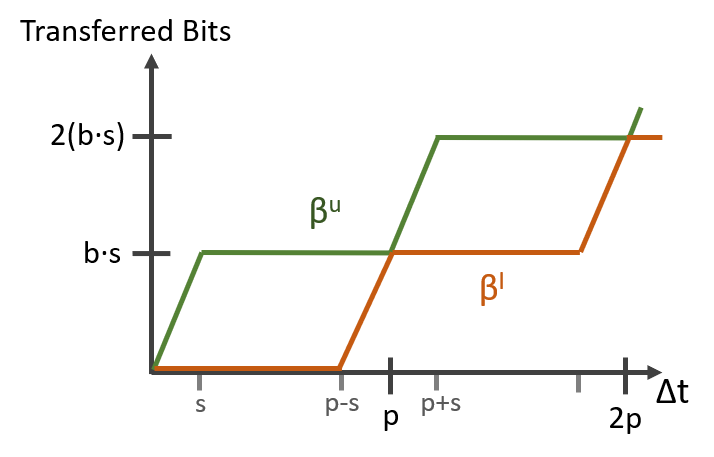
\includegraphics[width=0.8\columnwidth]{graphics/tdma_bus.png}
    \caption{Service curve of a simple TDMA bus}\label{fig:tdma_bus}
\end{figure}

\mysubsection{Service Curves of the Sample System}

Here we choose to use fully available CPUs as computational resources, with 4 or 5 million executable instructions per second (\textbf{MIPS}),
Additionally we use a TDMA bus as a communicational resource.
The available service of the bus is given by the bandwidth of 20 kilobits of transferrable information per second (\textbf{kbps}), a period of 10 and a slot length of 8.
The service curves of these resources are given by \autoref{fig:b-ins}.

\begin{figure}
    \centering
    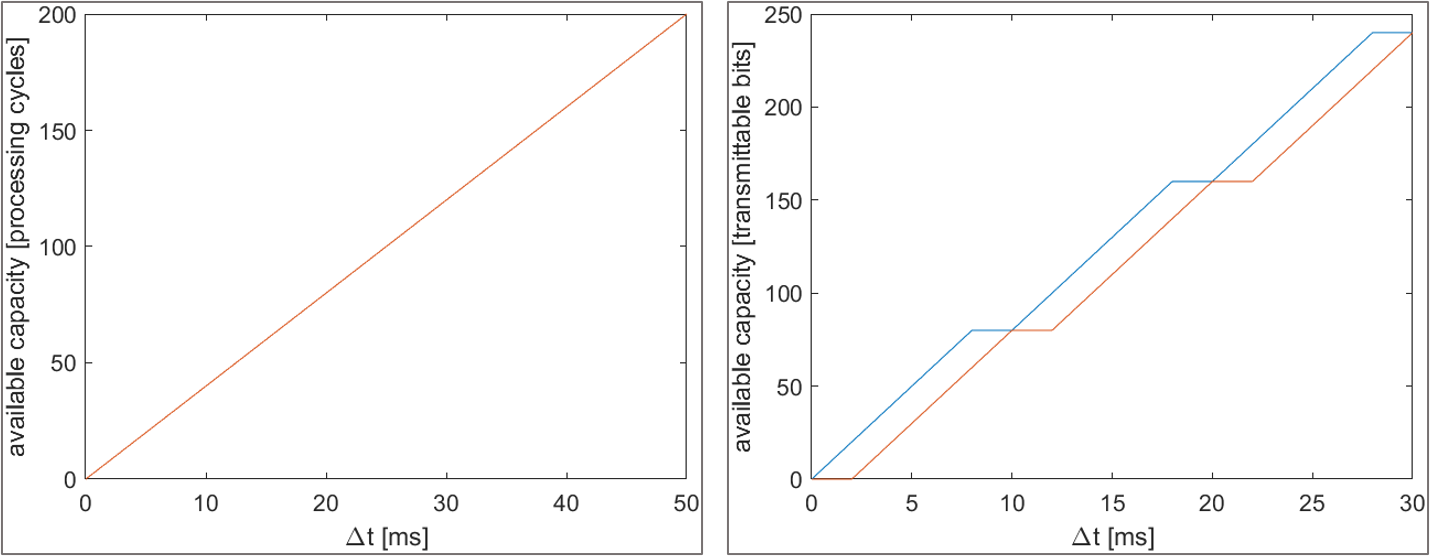
\includegraphics[width=\columnwidth]{graphics/example_b_ins.png}
    \caption{Service curves of the sample system's 4 MIPS CPU (left) and it's TDMA bus (right)}\label{fig:b-ins}
\end{figure}
\mysection{HW/SW-Components}\label{component}

A real-time embedded system consists of components, that provide the service capacity of the resources to the event streams, in order to give them the supplies they need for
executing their tasks.
Whenever an event stream now arrives at a computational or communicational component, an application task is interpreted and executed~\cite{wan:06}.
This processing usually leads to changes in the event arrival and service curves.
So how can we derive the properties of the outgoing streams \(\alpha'\) and \(\beta'\) from the properties of the incoming streams \(\alpha\) and \(\beta\)?

Let's suppose we have a simple system with only one single event stream arrival curve \(\alpha\) and one resource with service capacity \(\beta\) like in \autoref{fig:single_GPC}~\cite{ver}~\cite{thi:00}.

\begin{figure}
    \centering
    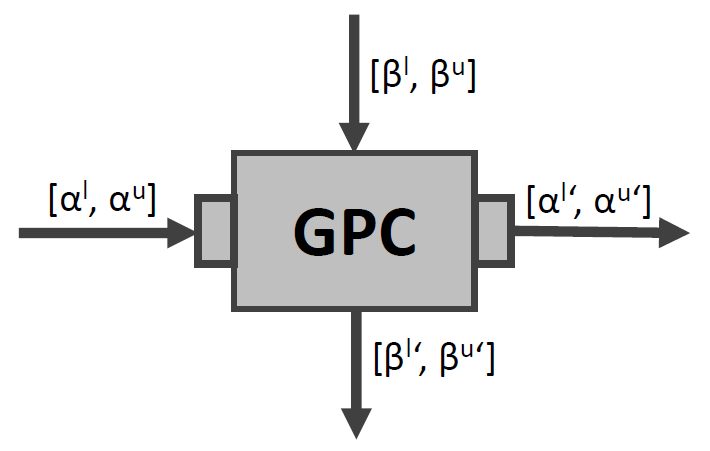
\includegraphics[width=0.7\columnwidth]{graphics/single_GPC.png}
    \caption{Single GPC with its incoming and outgoing streams}\label{fig:single_GPC}
\end{figure}

The pair of output arrival curves describes the event rates after this processing step, while the pair of output service curves describes the remaining service capacity~\cite{wan:06}.
The relations between \(\alpha, \beta, \alpha' \text{ and } \beta'\) and thereby the values of \(\alpha' \text {and } \beta'\) depend on the processing semantics of the component.
In general, they can be modeled as
\[ \alpha' = f_\alpha (\alpha, \beta)\] 
\[\beta' = f_\beta (\alpha, \beta) \]
where the function \textbf{f} is given for each component specifically and
depends on the processing semantics of the modeled component~\cite{wan:06}.
These processing semantics need to be provided in the application or resource description.

In the framework of MPA we are mostly working with abstract components.
Here the input and output streams are no concrete traces, but always just upper and lower borders for possible traces, like for example \(\alpha' = [\alpha'^{\, u}, \alpha'^{\, l}]\)~\cite{wan:06}.

Greedy processing components (\textbf{GPC}) are a common example for such components in real-time embedded systems.
A GPC is triggered by an incoming event, directly instantiates a task and then processes the event, and thereby its task, in a greedy fashion
in first-in-first-out order~\cite{cho:08}.
Of course this process is restricted by the resource availability \(\beta\).
The main advantage of using GPCs is, that we can easily compute the semantics of the component using the min/max-plus algebra (see \autoref{minMaxPlus})~\cite{wan:06}.
Thus, we will from now on assume that all of the components in this paper are GPC.

With a GPC the resulting event streams are~\cite{wan:06}:
\[\alpha'^{\, u} = \min \left\{ (\alpha^{u} \otimes \beta ^{\, u}) \oslash \beta^{\, l}, \beta^{\, u} \right\} \]
\[\alpha'^{\, l} = \min \left\{ (\alpha^{l} \oslash \beta ^{\, u}) \otimes \beta^{\, l}, \beta^{\, l} \right\} \]
While the remaining service capacities are:
\[\beta \, ^{\prime\, u} = (\beta ^{\, u} - \alpha ^{l}) \overline{\oslash} 0 \]
\[\beta \, ^{\prime\, l} = (\beta ^{\, l} - \alpha ^{u}) \overline{\otimes} 0 \]
\mysection{Constructing the System Performance Model}\label{complexSystem}

Usually a system needs more than just one component.
Therefore, a clever way to systematically link all those different components together is needed, as
we want to enable resource sharing, as well as a pipelined stream of data, in the system performance model.
This can be done by aligning multiple resources horizontally and multiple event streams vertically~\cite{wan:06}.

\mysubsection{Flow of Data}

Each event stream is typically processed by a sequence of HW/SW components.
The horizontal order of the steams determines the order, in which the event streams will pass by the resources~\cite{wan:06}.
At every intersection between an event and a resource stream, a component will be instantiated, in case that event stream needs to fulfil a task at this resource.

\mysubsection{Resource Sharing --- Impact of different Scheduling Policies}\label{scheduling}

An important step for designing a real-time embedded system is choosing a scheduling scheme for the resources,
as there are usually several event streams that need to use the same component at one time.
In the framework of MPA, various scheduling and arbitration policies can be used, like for example  
fixed priority, proportional share, TDMA, generalized processor sharing or earliest deadline first scheduling~\cite{wan:06}.
All of these policies have different techniques to distribute the available resources, in particular the remaining service capacities \(\beta'\), among the event streams in need.

Earlier, different approaches were needed when analyzing different classes of arbitration strategies, such as dynamic, static or hierarchical ones, as their event bounds need to be characterized in complete different ways.
Yet since~\cite{slo} there is a unified request bound available for all kinds of analysis purposes in real-time scheduling theory.
Therefore, the response time analysis can now be done with the same unified equation, identically what arbitration strategy is used in the system.

Following there are some examples of common scheduling policies and their uses in MPA.\

\mysubsubsection{Preemptive Fixed Priority Scheduling}

In a system with a fixed priority scheduling strategy, the processor always executes the task with the highest priority of the queue first. 
As those priorities are static, they do not change during execution time.
A preemptive scheduler additionally has a clock and will stop the execution of the task after a certain amount of time units have passed, to put the task back
into the queue and continue with the next one.
Meanwhile, a non-preemptive scheduler does never interrupt the execution of tasks and lets them run until they voluntarily unblock the processor again~\cite{mar}.

In preemptive fixed priority scheduling, tasks are preempted by higher priority tasks~\cite{slo}.
The vertical order of the event streams within the system model determines which event stream will get the highest service capacity and therefore determine the priorities of the event streams~\cite{wan:06}.
In general urgent or highly frequent tasks should be prioritized.
The lower priority event streams below can then only use the remaining service capacity to fulfill their tasks at the same processor~\cite{mar}.
As MPA is especially suitable for modeling fixed priority scheduling, this will be the primary used scheduling technique of the paper.

\mysubsubsection{Non-Preemptive Fixed Priority Scheduling}

Fixed priority scheduling with a non-preemptive strategy can also be used in the framework of MPA, yet
the integration into the system model is more complex than integrating its preemptive equivalent.
However, since~\cite{cho:08} and~\cite{sof:12/1} efficient and sufficiently general approaches are known 
to analyze systems with such arbitration behavior.
Still it is not possibly to just simply use GPUs here, as the components are not supposed to just process all inputs in a greedy manner one after another.
Instead, there is the need for abstracting the scheduling strategy from the system-level components like shown in \autoref{fig:scheduling-unit}.

\begin{figure}
    \centering
    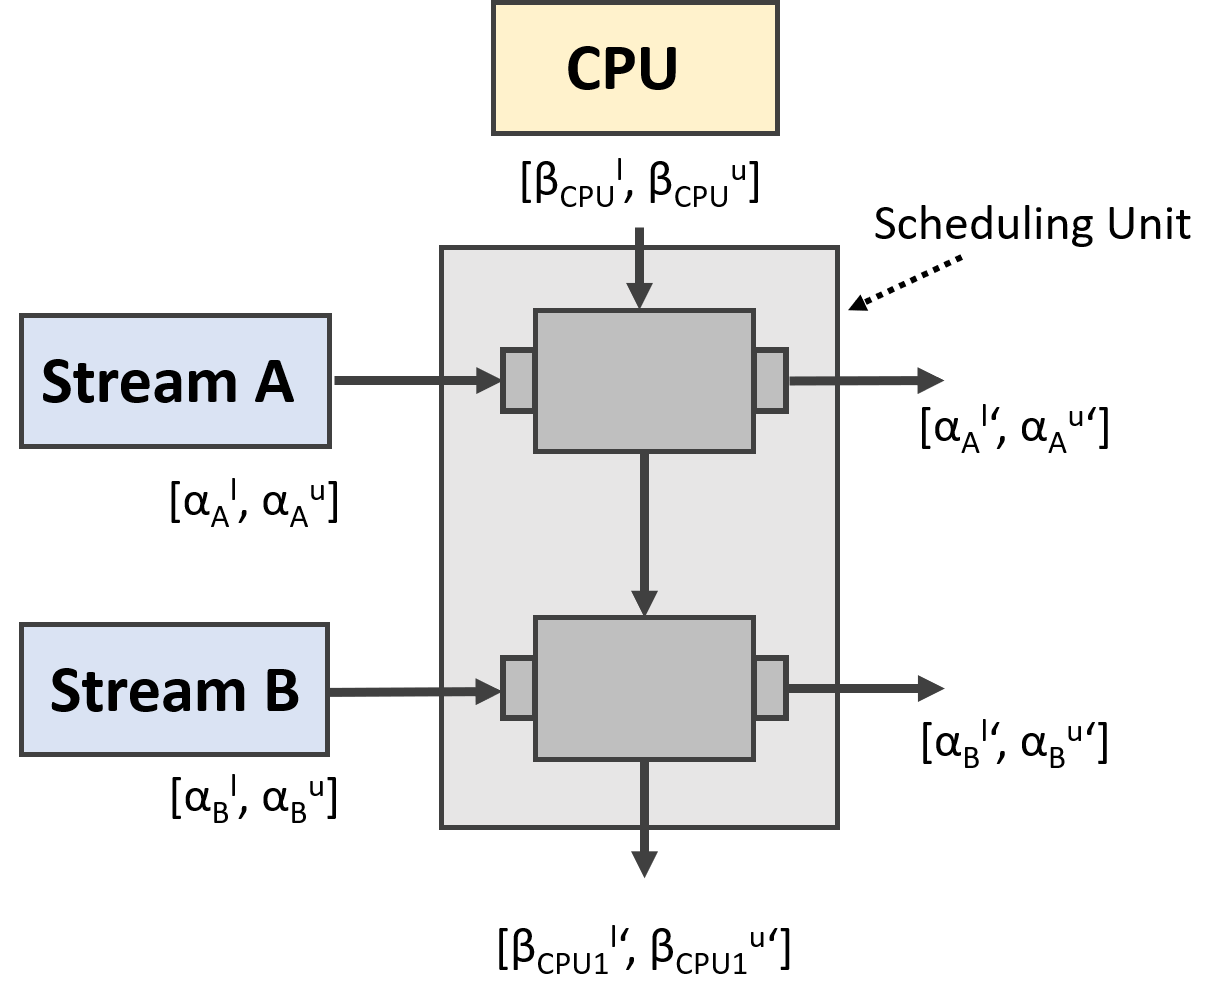
\includegraphics[width=0.8\columnwidth]{graphics/scheduling_unit.png}
    \caption{System Performance Model scheduled using a more complex arbitration technique. This could for example be Fixed Priority Non-Preemptive or Earliest Deadline First Scheduling. %
    The scheduling unit abstracts from the real components and manages what the component will process first.}\label{fig:scheduling-unit}
\end{figure}

\mysubsubsection{Earliest Deadline First Scheduling (\textbf{EDF})}

Similar to non-preemptive fixed priority scheduling, when using EDF scheduling, there is also the need to abstract the arbitration strategy from the components themselves (see \autoref{fig:scheduling-unit}).
Luckily there is great \href{https://www.mpa.ethz.ch/}{tool support} that allows us to treat EDF components just like any ``normal'' GPC.\
However, there now is the need to additionally include the deadline of every task into the calculation.
Using these deadlines, the demand bound function can be specified as the deadline shifted request bound function~\cite{slo}.

\mysubsection{System Performance Model of the Sample System}

Starting with the input data collected in \autoref{data} we can now construct a possible performance model of our system.
Here we decide to actually propose two different models in order to compare them later on: model A with two CPUs of 4 MIPS each connected by a bus (\autoref{fig:system-A}),
as well as model B of only one 5 MIPS CPU (\autoref{fig:system-B}).

After mapping the tasks to their corresponding resources using the information from \autoref{fig:seq_brightness} and \autoref{fig:seq_message}, we define all components to be GPCs.
As a scheduling technique we choose preemptive fixed priority scheduling and give the brightness event stream a higher priority than the
message event stream, as brightness events can occur more often and need quicker processing, in order for the system to seem responsive.

\begin{figure}
    \centering
    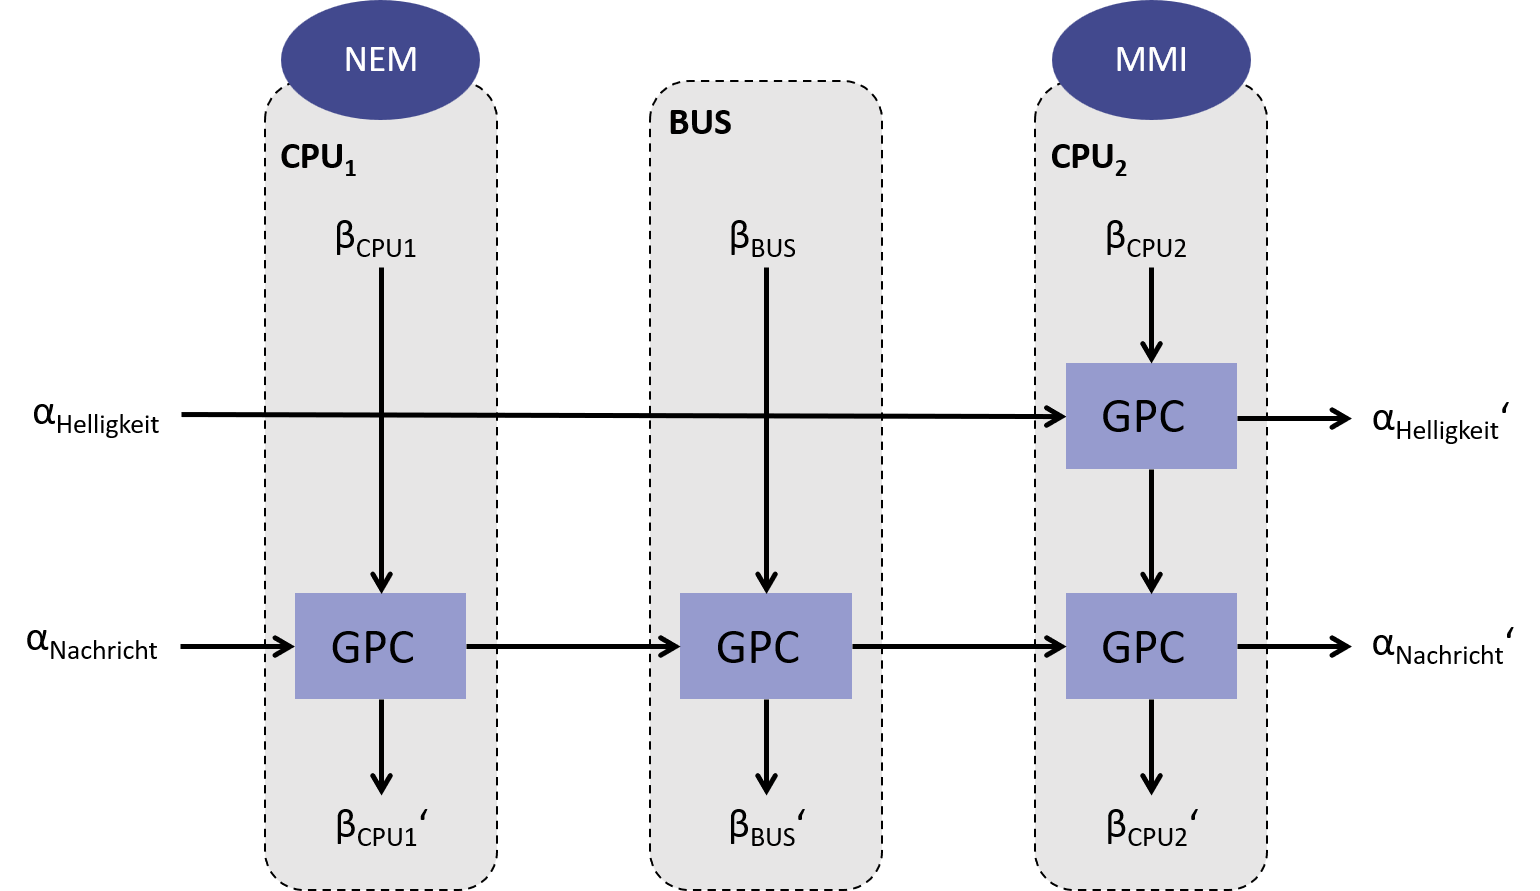
\includegraphics[width=\columnwidth]{graphics/system_A.png}
    \caption{System Performance Model of Architecture A}\label{fig:system-A}
\end{figure}

\begin{figure}
    \centering
    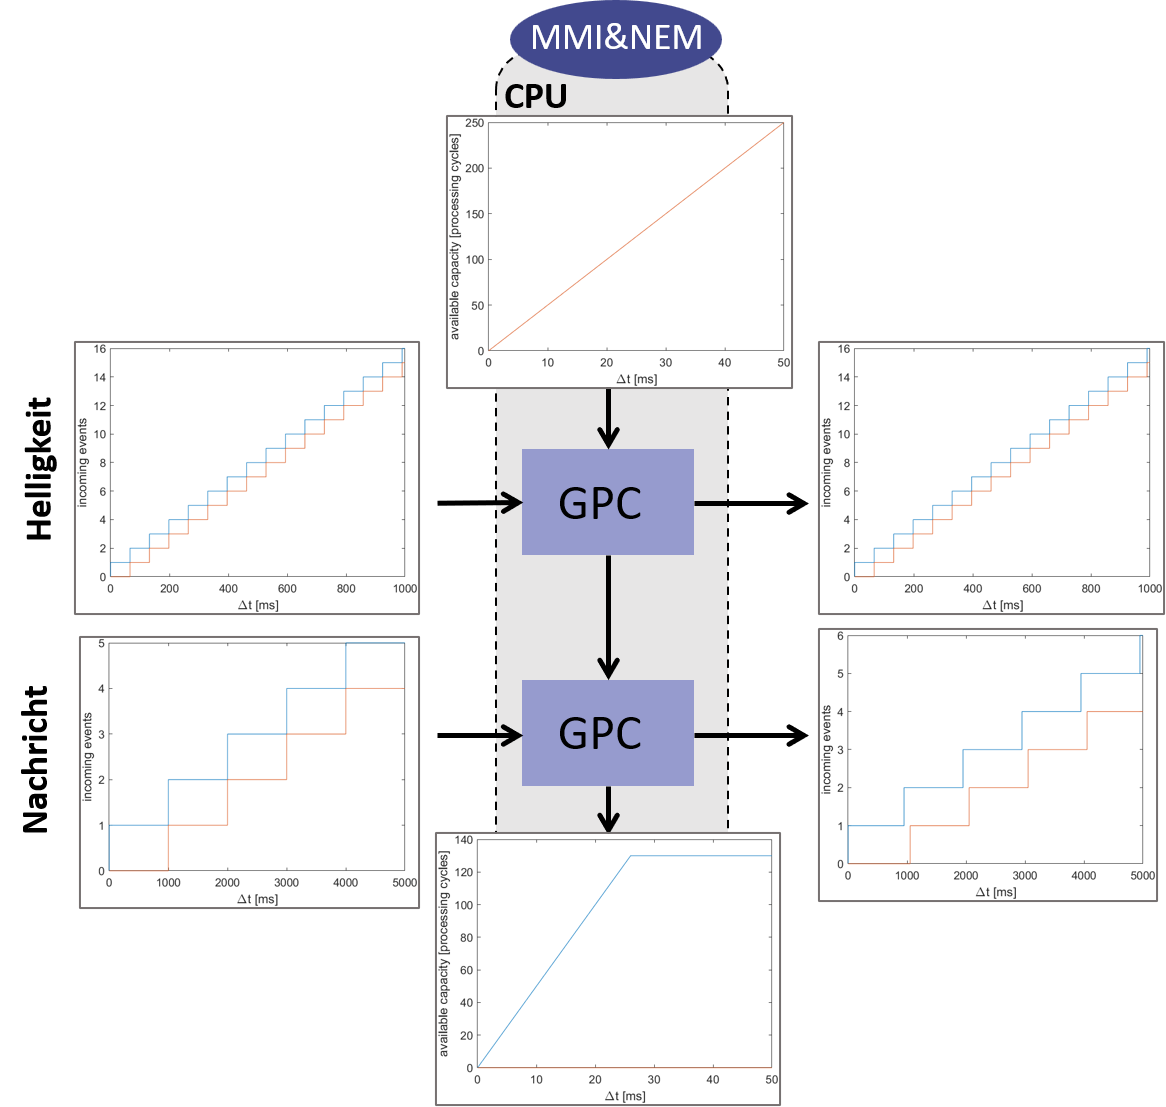
\includegraphics[width=0.9\columnwidth]{graphics/system_B.png}
    \caption{System Performance Model of Architecture A with the plotted input and output streams}\label{fig:system-B}
\end{figure}
\mysection{System Performance Analysis}\label{performanceAnalysis}

Now we can analytically evaluate the given system performance model regarding various performance criteria using MPA.\
The main assignment will be to find out, whether the system-level timing properties of this specific implementation meet the specified timing requirements~\cite{wan:05}.
The exact analysis methods may slightly vary for different abstract components, but always remains deterministic.
Following, the performance analysis methods for a system out of GPCs are presented.

The reason why the following equations use the Infimum and Supremum, instead of just using the minimum or maximum, can be found in~\cite{cru}.
Both, the delay and the buffer space calculations, consider \(\alpha ^{u}\) and \(\beta ^{\, l}\),
as \(d_{\max}\) and \(b_{\max}\) occur whenever the maximum load of events arrives at the time of minimum resource availability.
Visually these sizes can be interpreted as \autoref{fig:delays-vis}.

However, the system performance model is able to provide even more insights to a system.
For example analyzing the characteristics of the outgoing service curves, can expose the individual utilization of resources.
Besides that, the throughput of the event streams can also be calculated quite easily using the data of the system performance model~\cite{wan:06}.

\begin{figure}
    \centering
    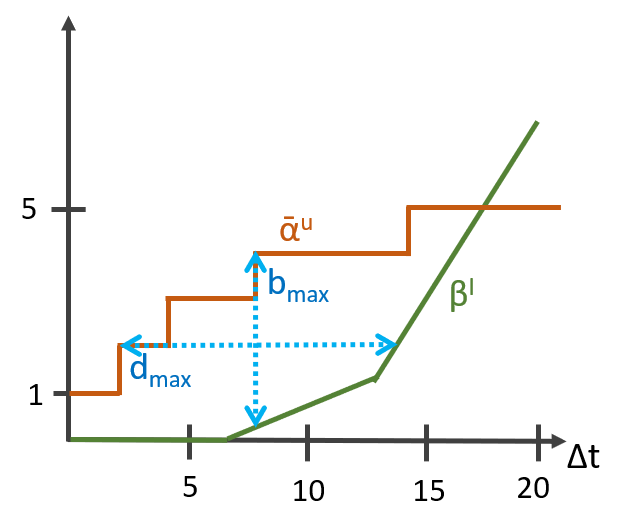
\includegraphics[width=0.7\columnwidth]{graphics/delays_vis.png}
    \caption{Graphically determining \(d_{\max}\) and \(b_{\max}\)}\label{fig:delays-vis}
\end{figure}

\mysubsection{Maximum Delay Guarantees}

The maximum delay \textbf{\(d_{\max}\)} experienced by any event on the event stream with arrival curve \(\alpha\) when being processed at a single GPC with service curve \(\beta\) is bounded by~\cite{cho:08}:
\[d_{\max} \leq Del (\alpha ^{u}, \beta ^{\, l})\]
\[Del (\alpha ^{u}, \beta ^{\, l}) := \sup_{\lambda \geq 0} \left\{ \inf_{\tau \geq 0}\left\{\alpha^{u}(\lambda) \leq \beta^{\, l}(\lambda+\tau)\right\}\right\}\]
The end-to-end delay experienced by an event with arrival curve \(\alpha\) that is being processed by \textbf{n} GPCs with the service curves \(\beta_{i}, \, i \in \{0, \ldots, n\}\) is furthermore bounded by:
\[d_{\max} \leq Del (\alpha ^{u}, \beta ^{\, l} _ 1 \otimes \cdots \otimes \beta ^{\, l} _n )\]
\[\leq Del (\alpha ^{u}, \beta ^{\, l} _1 ) + \cdots +  Del (\alpha ^{u}, \beta ^{\, l} _n ) \]
The calculation of the hard upper bounds to the maximum delays are quite conservative, yet they guarantee, that nothing every exceeds those bounds~\cite{cho:08}.

\mysubsection{Maximum Buffer Requirements}

We often also need to know how much storage space the internal buffers need, in order for them to always be able to temporarily store incoming events, that can not yet be processed.
This maximum required buffer space \textbf{\(b_{\max}\)} of a GPC with service curve \(\beta\) processing an event stream with arrival curve \(\alpha\) is bounded by~\cite{cho:08}:
\[b_{\max} \leq Buf \left(\alpha ^{u}, \beta ^{\, l}\right)\]
\[Buf \left(\alpha ^{u}, \beta ^{\, l}\right) := \sup _{\lambda \geq 0}\left\{\alpha^{u}(\lambda) - \beta^{\, l}(\lambda)\right\}\]
In the case of several consecutive tasks that all use the same shared memory, the required buffer space can be reduced to
\[b_{\max} \leq Buf (\alpha ^{u}, \beta ^{\, l} _ 1 \otimes \cdots \otimes \beta ^{\, l} _n )\] 
\[\leq Buf (\alpha ^{u}, \beta ^{\, l} _1) + \cdots +  Buf (\alpha ^{u}, \beta ^{\, l} _n ) \]

\mysubsection{Performance Analysis of the Sample System}

Both, architecture A and architecture B have the same buffer requirements.
In the sample system architecture A delays a brightness event by 50ms and a message event by 395ms.
Meanwhile, architecture B delays a brightness event by 40ms and a message event by 580ms.
As 580ms exceed the specified maximum delay of 500ms per message event, only architecture A is suitable for our scenario.
\mysection{System Sensitivity Analysis}\label{sensitivityAnalyis}

Next up we are going to find out how sensitive or robust the system is to a change in event input sizes.
Furthermore, we want to know where possible bottlenecks are and how to choose optimal processor or bus dimensions.

\mysubsection{How robust is the system?}

A robust system is not sensitive towards changes in the event stream rates:
An increase of the input data rate of any event stream by a few percents does not cause significant changes in the systems end-to-end delays~\cite{wan:06}.
Specifically the new end-to-end delays to not exceed the specified maximum delay times of the system applications.
In order to increase the system's robustness we need to look for and eliminate bottlenecks.

\mysubsection{Where is the bottleneck?}

The resource, that the system is most sensitive to, when changing its capacity, is a potential bottleneck resource.
If we now slightly higher the capacity of a bottleneck resource,
without chancing the capacities of any other resources, the end-to-end delay of at least one event stream immediately decreases, and therefore the system quality increases~\cite{wan:06}.

\mysubsection{Using the Results of MPA to Make Design Decisions: Improving Architectures}

When designing a new embedded real-time system, we want to find out what architecture works best for the specific use case.
Therefore, we want to try out numerous possible system models and compare them in therms of their performances and robustness.
\autoref{performanceAnalysis} and \autoref{sensitivityAnalyis} give us a great opportunities to do so, using the system performance model.
We can now quickly propose, analyze and compare various systems.
These systems may be extremely different, for example when trying out opposed architectures, or just slightly different, for example when decreasing a CPU's
performance by just a few percent to see if we can make the system cheaper, without risking any disadvantages.
Additionally, we can try out different scheduling strategies or change
the communication structure between the resources, to develop new, and thus maybe improved, system models~\cite{wan:06}.

In the end it is the goal to find a system that, fulfills the timing requirements of all applications
and is robust enough in respect to changes,
while being as cheap as possible and therefore as small-dimensioned as possible.

\mysubsection{Sensitivity Analysis of the Sample System}

After we chose architecture A to be sufficient to the timing requirements in \autoref{performanceAnalysis}, we now want to investigate on the
architecture's robustness and further improve it.
With \autoref{fig:robust-A} and \autoref{fig:robust-B} we realize that the architecture is actually quite robust to increasing event stream rates,
yet it is unable to handle more than 20 brightness events per second or more than 4 message events per second.

Increasing the capacities of CPU1 (\autoref{fig:bottleneck-B1}), the bus (\autoref{fig:bottleneck-B2}) or CPU2 (\autoref{fig:bottleneck-B3}),
all immediately lead to improved delays, at least when it comes to message events.
As the delays decrease the fastest, when increasing the resource capacity of CPU3, we choose this resource to be worthy of further improvements.

\begin{figure}
    \centering
    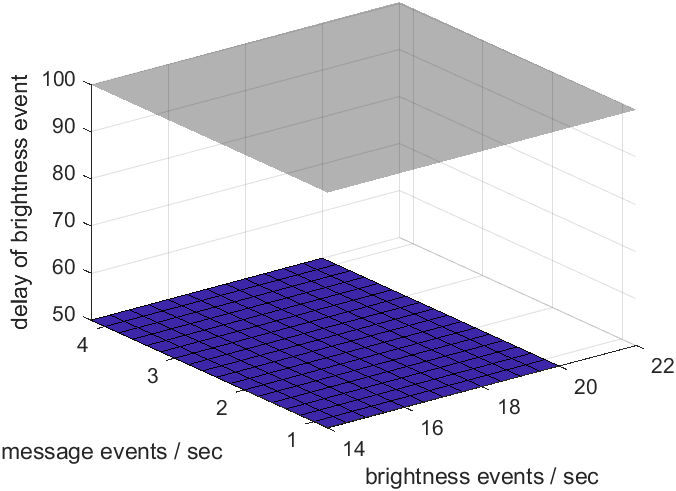
\includegraphics[width=0.8\columnwidth]{graphics/robustA.png}
    \caption{Impacts associated to increasing the rate of \(\alpha_{Brightness}\)}\label{fig:robust-A}
\end{figure}

\begin{figure}
    \centering
    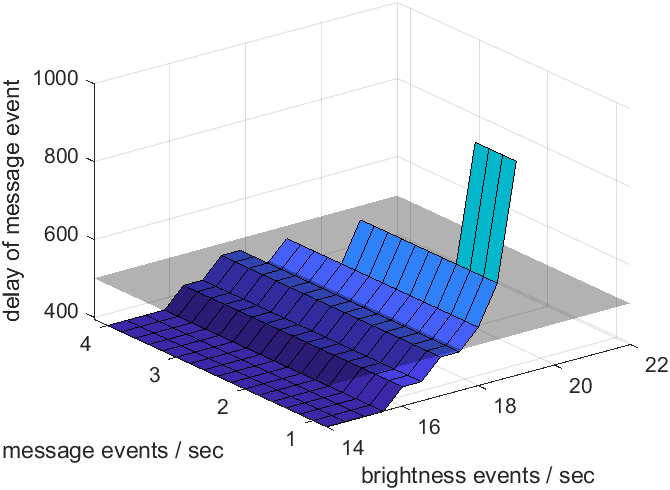
\includegraphics[width=0.8\columnwidth]{graphics/robustB.png}
    \caption{Impacts associated to increasing the rate of \(\alpha_{Message}\)}\label{fig:robust-B}
\end{figure}

\begin{figure}
    \centering
    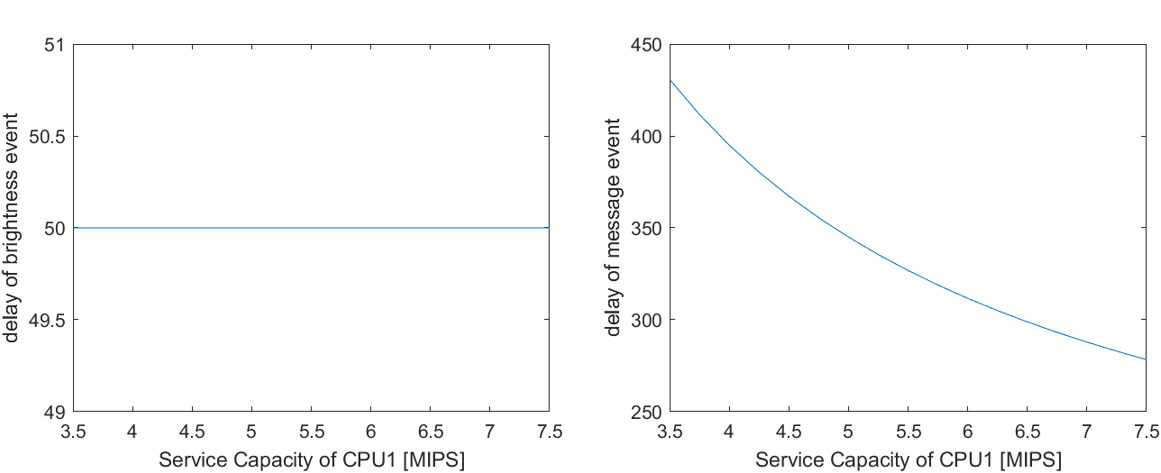
\includegraphics[width=\columnwidth]{graphics/bottleneckB1.png}
    \caption{Impacts associated to increasing the service capacity of CPU1}\label{fig:bottleneck-B1}
\end{figure}

\begin{figure}
    \centering
    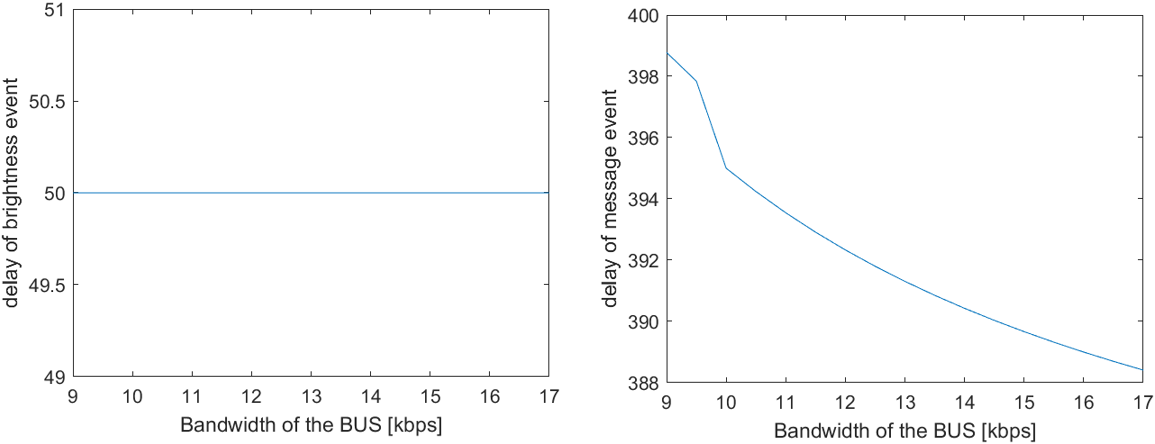
\includegraphics[width=\columnwidth]{graphics/bottleneckB2.png}
    \caption{Impacts associated to increasing the bandwidth of the BUS}\label{fig:bottleneck-B2}
\end{figure}

\begin{figure}
    \centering
    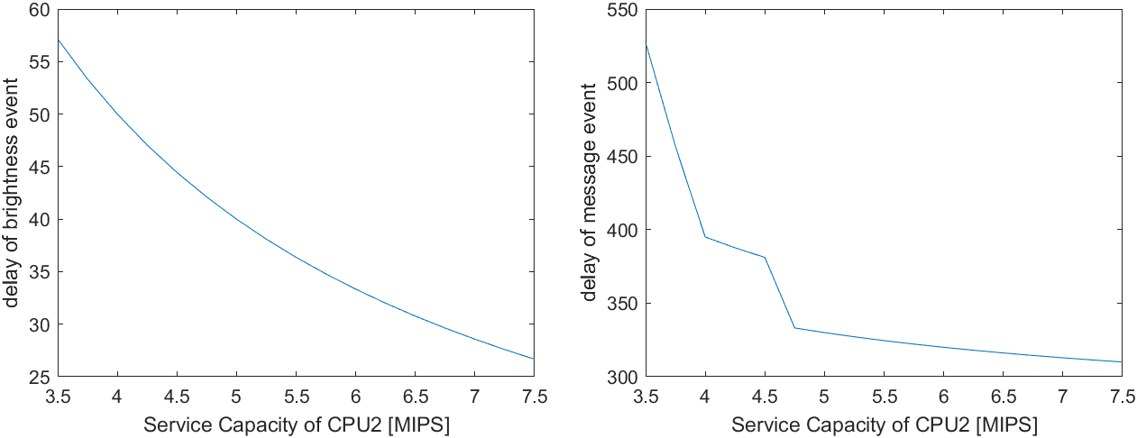
\includegraphics[width=\columnwidth]{graphics/bottleneckB3.png}
    \caption{Impacts associated to increasing the service capacity of CPU2}\label{fig:bottleneck-B3}
\end{figure}
\mysection{Discussion}\label{discussion}

\mysubsection{Advantages and Disadvantages of using a Formal Analysis Method}
In contrast to simulation based, probability based or holistic analysis methods for embedded real-time systems, formal methods can guarantee the correctness of their results~\cite{wan:06}.
The analysis will surely reveal the worst case bounds of system properties such as end-to-end delays.
Therefore, it is guaranteed that any system architecture accepted by the analysis, also fulfills all system requirements in reality~\cite{wan:06}.
On the other hand, system analysis using formal methods often leads to very pessimistic and in general not tight bounds, due to
a lack of details to include in the analysis and limited modeling capacities~\cite{wan:05}~\cite{cho:08}.
Using formal methods, we can only compute hard upper and lower bounds to the real system characteristics, which makes this method only suitable to analyze hard real-time systems only.
A system architecture might be rejected due to bad worst case guaranties, even if they are never actually reached
in execution and therefore the system in fact fulfills all requirements\cite{wan:06}.

Other significant advantages of the formal analysis are the fast analysis run-time, as well as the low set up effort for new architectures~\cite{wan:06}.
Similar models can be easily and quickly constructed and compared, as this merely involves reconnecting the event and service flows between the components.
In this way the technique is sufficiently productive even with a really high time-to-market pressure in the domain of embedded real-time systems and 
the interactive nature of the design process of such systems~\cite{ver}~\cite{hoo}.

Besides that, formal analysis methods are not suitable for systems with a dynamic and complex interactions, as this architecture can not be incorporated into the model properly~\cite{wan:06}.

\mysubsection{Advantages of Using MPA}

In contrast to many other formal analysis methods of embedded systems, the modular performance
analysis relies neither on standard arrival patterns of events, nor on classical scheduling~\cite{pha}.
In general the MPA can work really efficiently with only really few and abstract data about the system.
The low demand on detailed information, makes MPA a lightweight analysis method~\cite{wan:06}.
Furthermore, this leads to a high degree of generality and modularity, as well as an easy analyzability of system performance models~\cite{wan:06}.

The MPA and RTC framework is easy to use, especially when working with the \href{https://www.mpa.ethz.ch/}{RTC Toolbox for Matlab}.
It is a compositional method which simplifies the analysis of heterogeneous systems a lot.
In addition, MPA can represent the majority of different event arrival patterns, whether arbitrary or not~\cite{cho:08}.

\mysubsection{Disadvantages and Limitations of Using MPA}

As we are abstraction from the time domain to the time interval domain, it is
difficult to accurately exploit implicit timing correlations between event arrivals on different event streams within the MPA framework~\cite{wan:06}.

In MPA and RTC it is impossible to model state-dependent behavior, as state information cannot be modeled naturally. 
For example, scheduling policies, that depend on the fill-level of buffers just cannot be implemented in the framework of MPA.\
Yet, thanks to~\cite{pha} we can interface RTC curves with state-based models using automata and hence also model states in this new extended framework.
\mysection{Conclusion}\label{conclusion}

The framework of modular performance analysis proofs to be a powerful analyzing tool for hard distributed embedded real-time systems, 
that is capable of doing fast evaluations on system structures.
As shown in \autoref{discussion} using MPA with RTC has some major advantages and is useful for various contexts, 
especially for the use in early design phases of an embedded system to make important design decisions, as MPA can deal with only few and abstract information about the system~\cite{wan:06}.

The real-time calculus framework furthermore empowered MPA by formal analysis methods and efficient computation strategies for obtaining correct and accurate performance analysis results.
Even though the computed bounds on system performance characteristics, such as end-to-end delays and buffer requirements, are often quite pessimistic, they provide guaranteed hard bounds~\cite{wan:06}.

Although there are some limits to MPA and RTC, they both are really valuable approaches to the formal analysis during the design process of real-time embedded systems.
Therefore, they are still subjects of ongoing research.
Hence, there is a good chance, that some problems described in \autoref{discussion} will be solved at least partially within the next few years.

If enough information about the system and time to do the analysis are provided, it might also be an option to 
use MPA combined with a simulation based method for obtaining even better insights into the system~\cite{wan:06}.

\begin{appendices}
  \section{The Min/Max-Plus Calculus}\label{minMaxPlus}

Real-time calculus uses the min/max-plus algebra for computational purposes.
Instead of the usual algebraic structure of \((\mathbb{R},+,\cdot)\), we are now dealing with
\((\mathbb{R}\cup\infty,+,\cdot)\) as an algebraic structure. 
Luckily we do not need to deep dive into the characteristics of the algebra here, 
knowing and understanding the following operations on functions \(f\) and \(g\) is sufficient for being able to
use RTC as a calculation tool:

\begin{align*}
    \text{Min-Plus Convolution:} \\
    (f \otimes g)(\Delta t) &= \inf _{0 \leq \lambda \leq \Delta t} \left\{ f (\Delta t - \lambda) + g (\lambda) \right\} \\
    \text{Min-Plus Deconvolution:} \\
    (f \oslash g)(\Delta t) &= \sup _{\lambda \geq 0} \left\{ f (\Delta t + \lambda) - g (\lambda) \right\} \\
    \text{Max-Plus Convolution:} \\
    (f \overline{\otimes} g)(\Delta t) &= \sup _{0 \leq \lambda \leq \Delta t} \left\{ f (\Delta t - \lambda) + g (\lambda) \right\} \\
    \text{Max-Plus Deconvolution:} \\
    (f \overline{\oslash} g)(\Delta t) &= \inf _{\lambda \geq 0} \left\{ f (\Delta t + \lambda) - g (\lambda) \right\}
\end{align*}

Proofs and more detailed information on the min/max-plus algebra can be found in~\cite{bou}.
These equations can be quite complicated to compute,
but the \href{https://www.mpa.ethz.ch/}{RTC Toolbox for Matlab} is here to take care of them.
This toolkit is a great help when it comes to performing MPA for any kind of use case scenarios.

%As a reminder: The Supremum of a set of elements is defined as the set's least upper bound.
%In case it is within the set, the Supremum can be called a maximum.
%In an analogue way the Infimum of a set is defined as its greatest lower bound.
\end{appendices}

\bibliographystyle{IEEEtran}
\bibliography{IEEEabrv,references}

\end{document}